\documentclass{article} \usepackage{graphicx} \usepackage[utf8]{inputenc} \usepackage{polski} \author{C and bash} \title{Równiania}
 \begin{document} \maketitle
\begin{figure}
  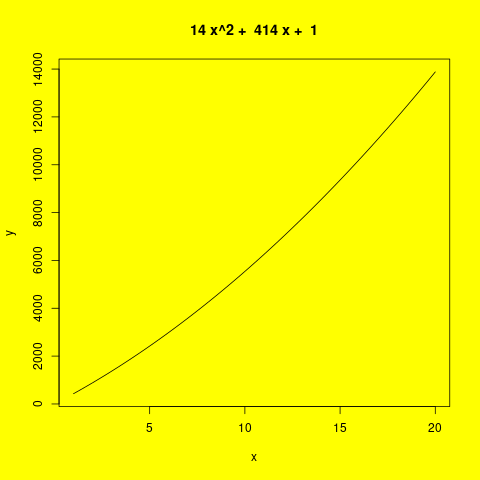
\includegraphics[width=\linewidth]{./tmp_charts/output.png}
  \caption{A boat.}
  \label{fig:boat1}
\end{figure}

\section{x^2*14+x*414+1} NEW \end{x^2*14+x*414+1}
NEW
\section{x^2*+x*+} NEW \end{x^2*+x*+}
NEW
\end{document}
